% ------------------------------------------------------------------
\renewcommand{\thisweek}{MATH327 Week 5}
\renewcommand{\moddate}{Last modified 27 Feb.~2021}
\setcounter{section}{5}
\setcounter{subsection}{0}
\phantomsection
\addcontentsline{toc}{section}{Week 5: Thermodynamic cycles}
\section*{Week 5: Thermodynamic cycles}
\subsection{Work, pressure and force}
Last week we defined the pressure in the canonical ensemble as the thermodynamic response of the internal energy to an adiabatic change in the volume (\eq{eq:pressure}).
At the same time, we motivated this definition by thinking about `squeezing' the system---exerting a force on it---which suggests a connection between pressure and force.
Here we make this connection explicit by considering how the energy of an object changes when a force acts on it.

\begin{shaded}
  Consider an object at position $\vec r = (x, y, z)$, and suppose it is displaced by a vector $d\vec r$ due to a force $\vec F(\vec r)$.
  The \textbf{work} done by this force is defined to be the resulting change in the energy of the object.
  Infinitesimally, $W = dE = \vec F\cdot d\vec r$, which generalizes to the line integral $W = \De E = \int \vec F(r)\cdot d\vec r$.
\end{shaded}

A famous example is an object falling due to the force of the Earth's gravity.
That force is $\vec F = (0, 0, -mg)$, where $m$ is the mass of the object, $g \approx 9.8~\mathrm{m}/\mathrm{s}^2$ (metres per second per second) is the strength of gravity near the surface of the Earth, and the negative sign indicates that the gravitational force is directed downward.
The object starts from rest, with initial (kinetic) energy $E_0 = 0$, and falls downward (parallel to $\vec F$) from a height $h$.
Its final energy $E_f$ upon hitting the ground comes from the work done by the Earth's gravity:
\begin{align*}
  W & = \int \vec F(r)\cdot d\vec r = -mg \int_h^0 dz = mgh > 0 \\
  E_f & = E_0 + \De E = 0 + W = mgh = \frac{p_z^2}{2m} \qquad \lra \qquad p_z = m\sqrt{2gh},
\end{align*}
where $\vec p = (p_x, p_y, p_z)$ is the momentum we considered last week (\eq{eq:momentum}).

To connect the concept of work to the pressure of a statistical system described by the canonical ensemble, let's consider the setup shown below (copied from Schroeder's \textit{Introduction to Thermal Physics}).
Here we have an gas in a container of volume $V$, with one wall of that container being a piston that we can displace by applying a force $F$.
Let's demand that this process is adiabatic---it does not change the entropy of the gas.
The displacement $\De x$ shown in the figure reduces the volume of the gas, by $\De V = -A\De x < 0$ where $A$ is the area of the piston.
Since the force $F$ is parallel to the piston's displacement $\De x$, it does positive work $W = F\De x > 0$.
Therefore the energy of the gas increases, at the same time as its volume decreases adiabatically, so from \eq{eq:pressure} we have
\begin{equation}
  P = -\left. \pderiv{}{V} \vev{E}\right|_S = -\frac{W}{\De V} = \frac{F\De x}{A\De x} = \frac{F}{A}
\end{equation}
This identifies the pressure of a gas in a container as the force per unit area that the gas exerts on the container wall, reassuringly consistent with our everyday experiences.

\begin{center}
  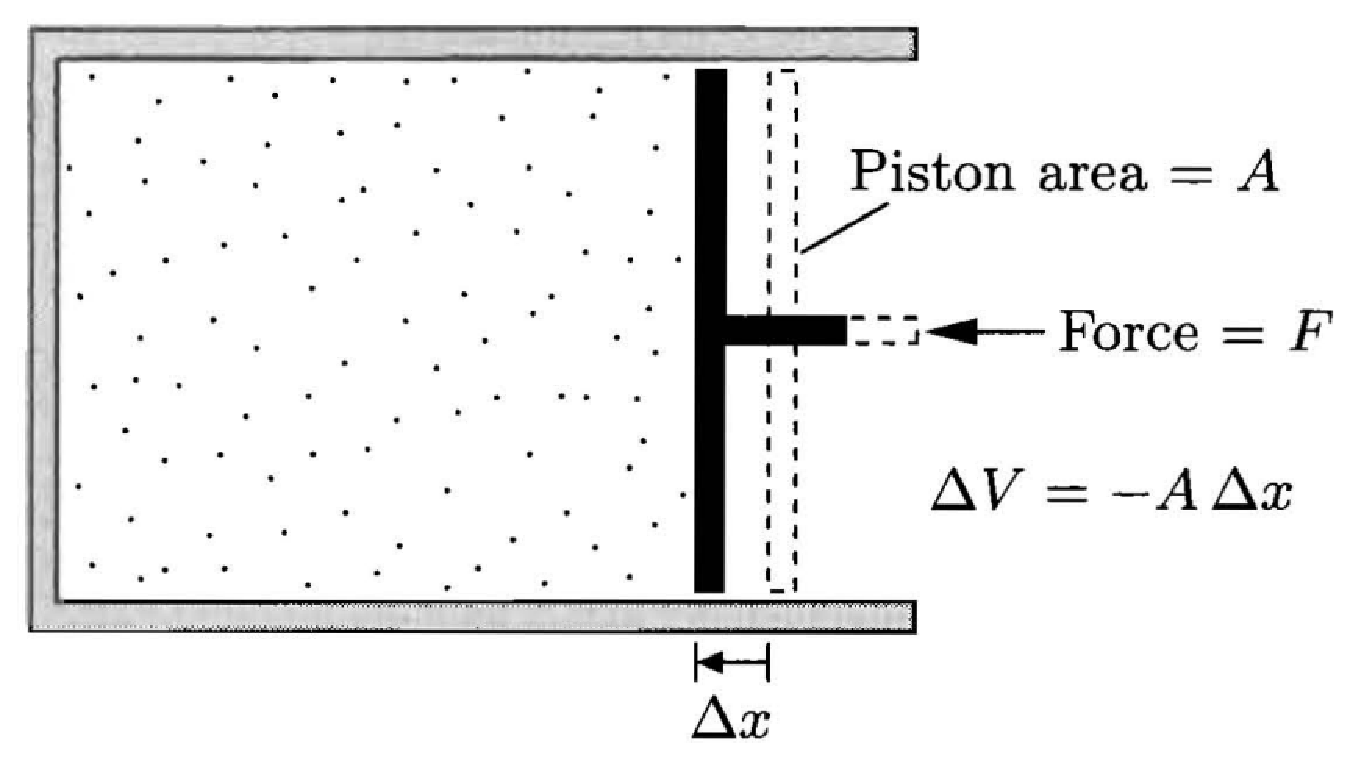
\includegraphics[width=0.7\textwidth]{figs/week05_piston.pdf}
\end{center}

Rearranging the expressions above, we can obtain an expression for the work \textit{put into} the gas by its surroundings (that is, by the external force applied to move the piston).
Still assuming an adiabatic (constant-entropy) process, this input work must match the increase in the gas's average internal energy,
\begin{align*}
  W_{\text{in}} & = \De \vev{E} = -P \De V & & \mbox{for constant entropy.}
\end{align*}
If the entropy is allowed to change, this relation between pressure and work will still hold---as we will see in the next section, we will simply no longer be able to identify the work as the total change in the average internal energy:
\begin{align}
  \label{eq:work_constP}
  W_{\text{in}} & = -P \De V & & \mbox{more generally.}
\end{align}
Later we will be interested in using the gas as a thermodynamic engine that \textit{does work on} its surroundings.
This removes energy from the gas, reversing the negative sign above, $W_{\text{done}} = -W_{\text{in}}$.

Of course, as we change the volume of the gas, the pressure itself will change as described by the gas's equation of state---such as the ideal gas law, \eq{eq:ideal_gas_law}.
With the equation of state providing an expression $P(V)$ for the pressure as a function of the volume, \eq{eq:work_constP} generalizes to
\begin{equation}
  \label{eq:work}
  W_{\text{in}} = -\int_{V_0}^{V_f} P(V) \; dV.
\end{equation}
% ------------------------------------------------------------------



% ------------------------------------------------------------------
\subsection{Heat and entropy}
Now let's switch things up by changing the temperature $T$ of an ideal gas while keeping its volume constant.
(As always for the canonical ensemble, the number of particles $N$ is also constant.)
Since the volume is constant, \eq{eq:work} indicates that no work is done, $W = 0$.
Even so, from \eq{eq:ideal_energy} we have $\vev{E} = \frac{3}{2} NT$ and can see that the average internal energy still changes,
\begin{equation}
  \label{eq:dE_dT}
  d\vev{E} = \frac{3}{2} N dT.
\end{equation}

In order to remain consistent with our discussion in the previous section, we should expect a change in the entropy to accompany this change in the internal energy that occurs with no work done.
Indeed, for both cases of distinguishable and indistinguishable particles, the temperature dependence of the entropy in \eq{eq:ideal_entropy} is the same:
\begin{equation*}
  S = N\log\left(\lath^{-3}\right) + T\mbox{-independent} = N\log\left(T^{3 / 2}\right) + T\mbox{-independent}.
\end{equation*}
What is the change in the entropy that results from changing the temperature by $dT$?
\begin{mdframed}
  $\displaystyle dS = $ \\[60 pt]
\end{mdframed}
Looking back to \eq{eq:dE_dT}, you should find $d\vev{E} = T dS$, which leads us to another important definition.

\begin{shaded}
  The \textbf{heat} added to or removed from a statistical system is defined to be
  \begin{equation}
    \label{eq:heat_def}
    Q = T dS,
  \end{equation}
  and corresponds to the change in the average internal energy of the system when the volume and particle number are kept constant.
\end{shaded}

Just as for the input work $W_{\text{in}}$ considered above, the heat $Q$ is positive if energy is added to the system to increase $\vev{E}$, and negative if energy is removed.
We are used to seeing the entropy as a derived function of the temperature, $S(T)$.
We can generally invert this relation to integrate over the infinitesimal\footnote{Sometimes infinitesimal heat and work are written $dQ$ and $dW$, but this invites misinterpretation as a `change' in heat or work, while the heat and work themselves are already changes in the internal energy.} definition in \eq{eq:heat_def},
\begin{equation}
  \label{eq:heat}
  Q = \int_{S_0}^{S_f} T(S) \; dS,
\end{equation}
with $Q = \De \vev{E}$ when the volume is constant.

This relation between heat exchange and changes in the entropy provides useful insight into what it means, physically, for a process to be adiabatic.
In order to keep the entropy constant, an adiabatic process has to occur with no heat moving into or out of the system.
In other words, \textbf{adiabatic processes are fast} enough that the system does not have time to exchange heat with its surroundings 
The opposite extreme would a process slow enough that any and all possible heat exchange can be completed while it is underway.
Based on our work in \secref{sec:heat_ex} we can see that such heat exchange will keep the system's temperature equal to the temperature of its surroundings.
Taking that surrounding temperature to be constant, we reach the conclusion that \textbf{constant-temperature (or isothermal) processes are slow}.
Most real processes exist in between these two extremes, usually closer to the adiabatic limit.
% ------------------------------------------------------------------



% ------------------------------------------------------------------
\subsection{Thermodynamic cycles}
Now we can generalize our work in the previous two sections to consider simultaneous changes in the temperature $T$ and the volume $V$ (still with fixed particle number $N$).
The internal energy $\vev{E}\!(T, V)$ and entropy $S(T, V)$ are functions of the temperature and volume, which provides relations that we can invert to express the temperature $T(S, V)$ and therefore the internal energy as functions of the entropy and volume,
\begin{equation*}
  \vev{E}\!(T, V) \to \vev{E}\!(S, V).
\end{equation*}
Expanding the internal energy to first order in a multi-variable Taylor expansion, we have
\begin{equation*}
  \vev{E}\!(S, V) \approx \vev{E}\!(S_0, V_0) + (S - S_0) \left.\pderiv{\vev{E}}{S}\right|_V + (V - V_0) \left.\pderiv{\vev{E}}{V}\right|_S.
\end{equation*}
This approximation becomes exact in the limit of infinitesimal changes, $(S - S_0) \to dS$, $(V - V_0) \to dV$ and $\vev{E}\!(S, V) - \vev{E}\!(S_0, V_0) \to d\vev{E}$.
At the same time, we can recognize the temperature from \eq{eq:temperature} and the (negative) pressure from \eq{eq:pressure}, to obtain
\begin{equation}
  d\vev{E} = T dS - P dV = Q + W_{\text{in}}.
\end{equation}
This is the general form of the \textbf{first law of thermodynamics}, with any change in the internal energy of a statistical system matched by (either or both) heat exchange with its surroundings or work done by or on those surroundings.

\begin{shaded}
  We now have all the conceptual tools and \textbf{key equations} needed to consider a variety of ways to manipulate an ideal gas in a container: \\
  \eq{eq:ideal_gas_law}
\end{shaded}

As examples, the piston shown in the figure above allows us to compress or expand the gas, and this change in volume can be either fast enough to keep the entropy constant (adiabatic) or slow enough to keep the temperature constant (isothermal).
Alternately, we can clamp the piston in place to keep the volume constant, and add heat to the gas to increase its temperature, which will also increase its pressure according to the ideal gas law.
We can also add heat while keeping the pressure constant (by applying a constant force to the piston), which 

If we 



%\TODO{key equations, PV diagrams, and repetition/cycling...}
\TODO{Being written...}
% ------------------------------------------------------------------



% ------------------------------------------------------------------
\newpage % TODO: Placeholder...
\subsection{The Carnot cycle}
\TODO{Being written...}
% ------------------------------------------------------------------
